\documentclass{beamer}
\usepackage{ctex, hyperref}
\usepackage[T1]{fontenc}

% other packages
\usepackage{latexsym,amsmath,xcolor,multicol,booktabs,calligra}
\usepackage{graphicx,pstricks,listings,stackengine}

\author{郑晖}
\title{A Thousand Brains}
\subtitle{A New Theory of Intelligence}
\institute{武汉大学弘毅学堂}
\date{2021年6月20日}
\usepackage{WHU}

% defs
\def\cmd#1{\texttt{\color{red}\footnotesize $\backslash$#1}}
\def\env#1{\texttt{\color{blue}\footnotesize #1}}
\definecolor{deepblue}{rgb}{0,0,0.5}
\definecolor{deepred}{rgb}{0.6,0,0}
\definecolor{deepgreen}{rgb}{0,0.5,0}
\definecolor{halfgray}{gray}{0.55}

\lstset{
  basicstyle=\ttfamily\small,
  keywordstyle=\bfseries\color{deepblue},
  emphstyle=\ttfamily\color{deepred},    % Custom highlighting style
  stringstyle=\color{deepgreen},
  numbers=left,
  numberstyle=\small\color{halfgray},
  rulesepcolor=\color{red!20!green!20!blue!20},
  frame=shadowbox,
}


\begin{document}

\kaishu
\begin{frame}
  \titlepage
  \begin{center}
    
\includegraphics[width=0.6\linewidth]{logo/logo.png}
  \end{center}
\end{frame}

\begin{frame}{Self Introduction}
  \begin{itemize}
    \item Hui Zheng
    \item Working on:
    \begin{itemize}
      \item the Neural Circuit Mechanisms of Cognition.
      \item Computational Neuroscience.
    \end{itemize}
    \item Co-advised by:
  \end{itemize}

  \begin{columns}
    \begin{column}{.2\linewidth}\end{column}
    \begin{column}{.3\linewidth}
      \begin{center}
        \includegraphics<1>[width=.6\linewidth]{figs/jingfengzhou.jpg}\\
        Dr. Jingfeng Zhou
      \end{center}
    \end{column}

    \begin{column}{.3\linewidth}
      \begin{center}
        \includegraphics<1>[width=.6\linewidth]{figs/yunzheliu.jpg}\\
        Dr. Yunzhe Liu
      \end{center}
    \end{column}
    \begin{column}{.2\linewidth}\end{column}
  \end{columns}
\end{frame}

\begin{frame}
  \tableofcontents[sectionstyle=show,subsectionstyle=show/shaded/hide,subsubsectionstyle=show/shaded/hide]
\end{frame}

\section{Background}

\subsection{About the Author}

\begin{frame}{About the Author}
  \begin{columns}
    \begin{column}{.7\linewidth}
      \begin{itemize}
        \item Jeff Hawkins
        \item Computer Scientist and Neuroscientist.
        \item At the 2021 BAAI Conference, he delivered a speech entitled「The Thousand Brains Theory - A roadmap for creating machine intelligence」.
      \end{itemize}
    \end{column}
 
    \begin{column}{.3\linewidth}
      \begin{center}
        \includegraphics<1>[width=.8\linewidth]{figs/jeff-hawkins.png}
      \end{center}
    \end{column}
  \end{columns}
\end{frame}

\subsection{Two Paths to AGI}
\begin{frame}{Two Paths to AGI}
  \begin{itemize}
    \item Focus on specificity: get computers to outperform humans on specific tasks.
    \item Focus on flexibility: create machines that can do many things and apply what they learn from one task to another.
  \end{itemize}
\end{frame}

\subsection{How to go from brain science to artificial intelligence?}
\begin{frame}{How to go from brain science to artificial intelligence?}
  \begin{itemize}
    \item Brain Science.
    \item Computational Neuroscience.
    \item Brain-Inspired Computing.
  \end{itemize}
  \begin{center}
    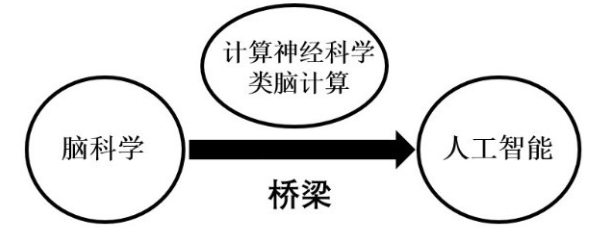
\includegraphics[width=0.6\linewidth]{figs/brain2ai.png}
  \end{center}
\end{frame}

\begin{frame}{Brain Science}
  \begin{columns}
    \begin{column}{.5\linewidth}
      \setbeamercolor{alerted text}{fg=red}
      \begin{itemize}
        \item<1-|alert@1> Electrophysiological recording.
        \item<2-|alert@2> Using cryo-electron microscopy images to reconstruct brain structure.
      \end{itemize}
    \end{column}

    \begin{column}{.5\linewidth}
      \includegraphics<1>[width=0.6\linewidth]{figs/electrophysiological-recording.png}
      \includegraphics<2>[width=0.8\linewidth]{figs/brain-reconstruct.png}
    \end{column}
  \end{columns}
\end{frame}

\begin{frame}{Computational Neuroscience}
  \begin{itemize}
    \item Neuronal Dynamics.
  \end{itemize}
  \begin{columns}
    \begin{column}{.1\linewidth}\end{column}
    \begin{column}{.4\linewidth}
      \begin{center}
        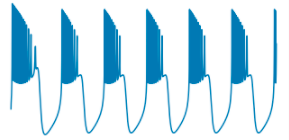
\includegraphics[width=0.6\linewidth]{figs/neuro-dynamics.png}\\
        Microscopic Phenomenon Modeling
      \end{center}
    \end{column}
    \begin{column}{.4\linewidth}
      \begin{center}
        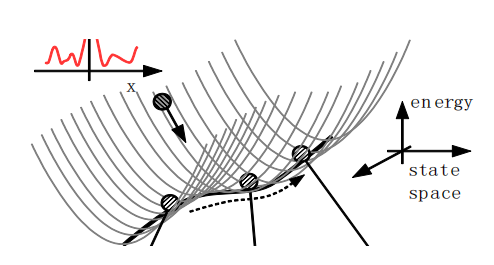
\includegraphics[width=0.6\linewidth]{figs/cann.png}\\
        Macroscopic Phenomenon Modeling
      \end{center}
    \end{column}
    \begin{column}{.1\linewidth}\end{column}
  \end{columns}
\end{frame}

\begin{frame}{Brain-Inspired Computing}
  \begin{columns}
    \begin{column}{.5\linewidth}
      \setbeamercolor{alerted text}{fg=red}
      \begin{itemize}
        \item<1-|alert@1> "Tianji" Chip.
        \item<2-|alert@2> SNN.
        \item<3-|alert@3> Dendritic Computing.
      \end{itemize}
    \end{column}

    \begin{column}{.5\linewidth}
      \begin{center}
        \includegraphics<1>[width=\linewidth]{figs/tianji-chip.png}
        \includegraphics<2>[width=0.6\linewidth]{figs/snn.png}
        \includegraphics<2>[width=0.6\linewidth]{figs/brainpy.jpg}
        \includegraphics<3>[width=0.6\linewidth]{figs/active-dendrites.png}
      \end{center}
    \end{column}
  \end{columns}
\end{frame}

\section{Neucortex}

\begin{frame}{The Composition of the Brain}
  \begin{columns}
    \begin{column}{.65\linewidth}
      \begin{itemize}
        \item \textbf{Neucortex}: One continuous sheet of neural tissue 70\% of brain by volume.
        \begin{itemize}
          \item Perception.
          \item Language.
          \item Cognition, thought, planning(engr., math, science, literature...)
        \end{itemize}
        \item \textbf{"Older" brain areas}: Dozens of specialized brain regions 30\% of brain by volume.
        \begin{itemize}
          \item Breathing, digestion, reflex behaviors.
          \item Walking, running, chewing.
          \item Emotions.
        \end{itemize}
      \end{itemize}
    \end{column}
 
    \begin{column}{.35\linewidth}
      \includegraphics<1>[width=\linewidth]{figs/brain.png}
    \end{column}
  \end{columns}
\end{frame}

\begin{frame}{The Neucortex Learns a Model of the World}
  \begin{columns}
    \begin{column}{.65\linewidth}
      \begin{itemize}
        \item Everything you know is stored in this model.
        \begin{itemize}
          \item How things look, feel, and sound.
          \item Where things are located.
          \item How things change when we interact with them.
          \item Includes tens of thousands of objects, words, and concepts.
        \end{itemize}
        \item The brain's model allows us to:
        \begin{itemize}
          \item Recognize objects and where we are.
          \item Predict the consequences of our actions.
          \item Plan and achieve goals.
        \end{itemize}
      \end{itemize}
    \end{column}
 
    \begin{column}{.35\linewidth}
      \includegraphics<1>[width=\linewidth]{figs/brain.png}
    \end{column}
  \end{columns}
\end{frame}

\begin{frame}{The Composition of the Neucortex}
  \begin{itemize}
    \item The Neurotex looks uniform.
    \item But it is divided into dozens of functional regions.
  \end{itemize}
  \begin{center}
    \includegraphics<1>[width=.6\linewidth]{figs/neucortex.png}
  \end{center}
\end{frame}

\begin{frame}{The Circuits of the Neucortex Look Similar Everywhere}
  \begin{columns}
    \begin{column}{.6\linewidth}
      \includegraphics<1>[width=\linewidth]{figs/neucortex-circuits.png}
    \end{column}
 
    \begin{column}{.4\linewidth}
      Common Circuitry
      \begin{itemize}
        \item Types of Neurons.
        \item Organized in layers.
        \item Connections between layers.
        \item Sensory input.
        \item Motor output.
      \end{itemize}
    \end{column}
  \end{columns}
\end{frame}

\begin{frame}{Vernon Mountcastle's Big Idea}
  \begin{itemize}
    \item All areas of the neucortex look the same because they perform the same intrinsic function. What makes one region visual and another auditory is what it is connected to.
    \item The human neucortex got large by copying a functional unit, the "cortical column".
  \end{itemize}
  \begin{center}
    \includegraphics<1>[width=.9\linewidth]{figs/cortical-column.png}
  \end{center}
\end{frame}

\section{The Thousand Brains Theory}

\begin{frame}{The Thousand Brains Theory}
  \setbeamercolor{alerted text}{fg=red}
  \begin{itemize}
    \item<1-|alert@1> Columns learn models by integrating sensory input and movement over time.
    \item<2-|alert@2> There are thousands of models for every object.
  \end{itemize}
  \begin{center}
    \includegraphics<1>[width=.4\linewidth]{figs/theory-1.png}
    \includegraphics<2>[width=.8\linewidth]{figs/theory-2.png}
  \end{center}
\end{frame}

\begin{frame}{The Composition of Column}
  Cortical columns create models using the same machanisms as grid cells and place cells use to model environments.
  \begin{center}
    \includegraphics<1>[width=.8\linewidth]{figs/column-composition.png}
  \end{center}
\end{frame}

\begin{frame}{Experimental evidence}
  \begin{itemize}
    \item Grid cells exist in pre-frontal cortex, used to model concepts.
    \begin{center}
      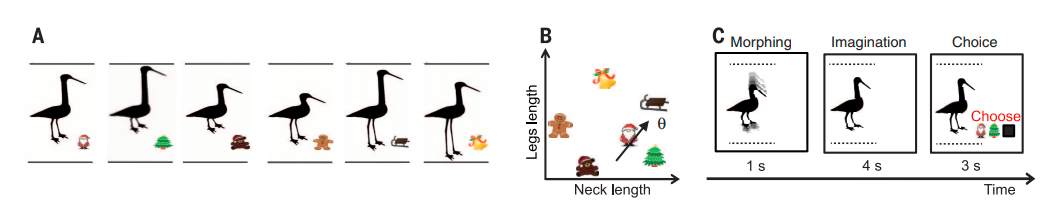
\includegraphics[width=.8\linewidth]{figs/ofc-gridlike.png}
    \end{center}
    \item Grid cells, place cells, border cells in Somatosensory cortex.
    \begin{center}
      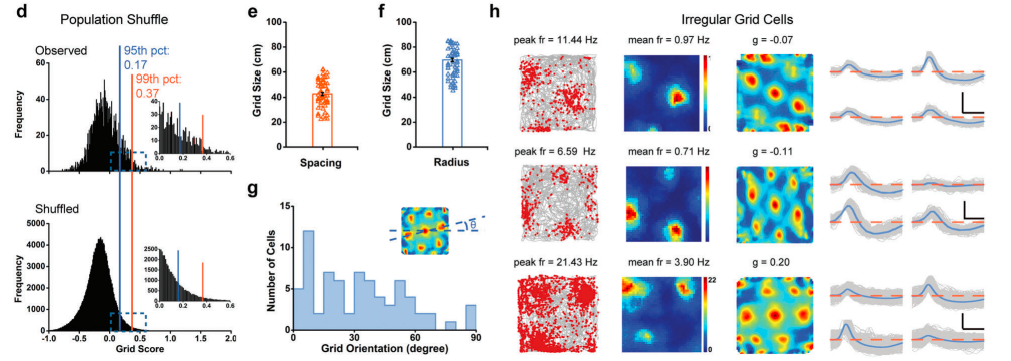
\includegraphics[width=.8\linewidth]{figs/novel-somasensory.png}
    \end{center}
  \end{itemize}
\end{frame}

\section{Roadmap}

\begin{frame}{A Roadmap for Creating Machine Intelligence}
  \begin{columns}
    \begin{column}{.1\linewidth}\end{column}
    \begin{column}{.4\linewidth}
      \setbeamercolor{alerted text}{fg=red}
      \begin{itemize}
        \item<1-|alert@1> Sparsity.
        \item<2-|alert@2> Active Dendrites.
        \item<3-|alert@3> Reference Frames.
        \item<4-|alert@4> Cortical Columns.
      \end{itemize}
    \end{column}
    \begin{column}{.4\linewidth}
      \includegraphics<1>[width=\linewidth]{figs/sparsity.png}
      \includegraphics<2>[width=\linewidth]{figs/active-dendrites.png}
      \includegraphics<3>[width=\linewidth]{figs/reference-frames.png}
      \includegraphics<4>[width=\linewidth]{figs/cortical-columns.png}
    \end{column}
    \begin{column}{.1\linewidth}\end{column}
  \end{columns}
\end{frame}

\begin{frame}{Thanks}
  \begin{itemize}
    \item Thanks for listening!
    \item Q\&A.
  \end{itemize}
\end{frame}

\end{document}
